\documentclass[11pt]{article}

\usepackage[letterpaper]{geometry}
%\usepackage[letterpaper,left=2.5cm,top=2cm,right=2.5cm,bottom=2cm]{geometry}

\usepackage[utf8]{inputenc}
\usepackage{mathpazo}
\usepackage{amsmath}
\usepackage{amsfonts}
\usepackage{siunitx}
\usepackage{cancel}

\usepackage{graphicx}
\usepackage{float}
\usepackage{empheq}
\usepackage[most]{tcolorbox}

\newtcbox{\mymath}[1][]{%
  nobeforeafter, math upper, tcbox raise base,
  enhanced, colframe=black!30!black,
  colback=yellow!30, boxrule=1pt,
  #1}

% Hyperlinks with decent looking default colors.
\usepackage{hyperref}
\usepackage{xcolor}
\hypersetup{
  colorlinks,
  linkcolor={red!50!black},
  citecolor={blue!50!black},
  urlcolor={blue!80!black}
}

% For those sexy spaced low small caps from classic-thesis!
\usepackage{microtype}
\usepackage{textcase}
\DeclareRobustCommand{\spacedlowsmallcaps}[1]{%
  \textls[80]{\scshape\MakeTextLowercase{#1}}%
}

% Replaced mathpazo \sum symbol with computer modern's.
\DeclareSymbolFont{cmlargesymbols}{OMX}{cmex}{m}{n}
\let\sumop\relax
\DeclareMathSymbol{\sumop}{\mathop}{cmlargesymbols}{"50}

\newcommand{\forceindent}{\leavevmode{\parindent=1em\indent}}

\usepackage{fancyhdr}
\pagestyle{fancy} 
\fancyhead{}
\rhead{Ali Ramadhan}
\lhead{6.339 Project 2---Finite Volume Methods}
\cfoot{\thepage}

\title{\spacedlowsmallcaps{6.339: Numerical Methods for Partial Differential Equations}\\ \spacedlowsmallcaps{Project two: Finite Volume Methods}}
\author{Ali Ramadhan$^\text{†}$ (\texttt{alir@mit.edu})}
\date{\textit{$^\text{†}$Department of Earth, Atmospheric, and Planetary Sciences}}

\renewcommand\thesection{\Alph{section}}

\begin{document}
\maketitle

In this project, we will utilize finite volume methods to study dense traffic flow and traffic jams modeled as shockwaves. We model traffic in each lane by a scalar hyperbolic conservation law, following what is known as the Lighthill-Whitman-Richards model.

We use a scalar hyperbolic conservation law to model traffic density $\rho^{(\ell)}(x,t)$ for $n$ lanes indexed by $\ell = 1,2,\dots,n$
\begin{equation} \label{eq:conservationLaw}
	\frac{\partial \rho^{(\ell)}}{\partial t} + \frac{\partial (\rho^{(\ell)} v^{(\ell)})}{\partial x} = s
\end{equation}
where $v^{(\ell)}(x,t)$ is the average velocity of the cars. This, however, provides us with only one equation for two unknowns and thus we specify the velocity by
\begin{equation} \label{eq:velocity}
	v(\rho) = v_\mathrm{max} \left( 1 - \frac{\rho^2}{\rho_\mathrm{max}^2} \right)
\end{equation}
giving us a traffic flux of 
\begin{equation} \label{eq:flux}
f(\rho) = \rho v = v_\mathrm{max} \left( \rho - \frac{\rho^3}{\rho_\mathrm{max}^2} \right)
\end{equation}
The source term
\begin{equation} \label{eq:source}
	s^{(\ell)} = \sumop_{\substack{|k-\ell|=1 \\ 1 \le k,\ell \le n}} \alpha \left( \rho^{(k)} - \rho^{(\ell)} \right)
\end{equation}
models the density of traffic that is switching lanes from neighboring lanes. $\alpha$ is the fraction of drivers that change lanes.

We will split up our one-dimensional grid into a number of cells indexed by $i=1,2,\ldots,N$. We will index the edges of the cell $i$ by $i-\frac{1}{2}$ for the left boundary of the cell, and by $i+\frac{1}{2}$ for the right boundary of the cell. So we can think of $i$ as indexing the cell centers.

To derive a first-order conservative finite-volume scheme for a single lane, we will consider the volume averages of the traffic density $\rho(x,t)$ at two different times. The volume average of the traffic density at cell $i$, $\rho_i = \rho(x_i,t)$, at a time $t_1$ over $x \in \left[ x_{i-\frac{1}{2}}, x_{i+\frac{1}{2}} \right]$ must exist by the mean value theorem and is given by
\begin{equation*}
	\bar{\rho}_i(t_1) = \frac{1}{\Delta x_i} \int_{x_{i-\frac{1}{2}}}^{x_{i+\frac{1}{2}}} \rho(x,t_1) \; dx
\end{equation*}
and an identical expression can be written for the volume average at a later time $t_2 > t_1$. Now, integrating the scalar conservation law in time from $t = t_1$ to $t = t_2$ we can write
\begin{equation*}
	\int_{t_1}^{t_2} \frac{\partial\bar{\rho}}{\partial t} \; dt + \int_{t_1}^{t_2} \frac{\partial(\bar{\rho} v)}{\partial x} \; dt = 0
\end{equation*}                         
where the first integral can be evaluated using the second fundamental theorem of calculus, sometimes referred to as the Newton–Leibniz axiom, and rearranged to obtain $\bar{\rho}_i$ at a later time
\begin{equation*}
\bar{\rho}(x,t_2) = \bar{\rho}(x,t_1) - \int_{t_1}^{t_2} \frac{\partial(\bar{\rho}_i v_i)}{\partial x} \; dt
\end{equation*}

We can now calculate $\rho_i(t_2)$ as
\begin{align*}
\bar{\rho}_i(t_2) &=
	\frac{1}{\Delta x_i} \int_{x_{i-\frac{1}{2}}}^{x_{i+\frac{1}{2}}} \left[ \rho(x,t_1) - \int_{t_1}^{t_2} \frac{\partial(\rho v)}{\partial x} \; dt \right] \; dx \\
	&= \frac{1}{\Delta x_i} \int_{x_{i-\frac{1}{2}}}^{x_{i+\frac{1}{2}}} \rho(x,t_1) \; dx - \frac{1}{\Delta x_i} \int_{x_{i-\frac{1}{2}}}^{x_{i+\frac{1}{2}}} \int_{t_1}^{t_2} \frac{\partial(\rho v)}{\partial x} \; dt \; dx \\
	&= \bar{\rho}_i(t_1) - \frac{1}{\Delta x_i} \int_{t_1}^{t_2} \left[ \rho(x_{i+\frac{1}{2}}, t) v(x_{i+\frac{1}{2}}, t) - \rho(x_{i-\frac{1}{2}}, t) v(x_{i-\frac{1}{2}}, t) \right] \; dt \\
	&= \bar{\rho}_i(t_1) - \frac{1}{\Delta x_i} \left[ \int_{t_1}^{t_2} F_{i+\frac{1}{2}} - F_{i-\frac{1}{2}} \right] \; dt
\end{align*}
which can be rearranged to write
\begin{equation*}
	\bar{\rho}_i(t_2) - \bar{\rho}_i(t_1) = \frac{d}{dt} \int_{t_1}^{t_2} \rho_i(t) \; dt = \int_{t_1}^{t_2} \left( - \frac{F_{i+\frac{1}{2}} - F_{i-\frac{1}{2}}}{\Delta x_i} \right) \; dt
\end{equation*}
where the integrands inside the two integrals must be the same so that
\begin{equation*}
	\frac{d \bar{\rho}_i}{dt} = - \frac{F_{i+\frac{1}{2}} - F_{i-\frac{1}{2}}}{\Delta x_i}
\end{equation*}
and if we approximate the time derivate by a first-order forward difference finite difference operator $\dot{\bar{\rho}}_i = (\bar{\rho}_i^{n+1} - \bar{\rho}_i^n)/\Delta t$ and further rearrange, we obtain
\begin{equation}
	\bar{\rho}_i^{n+1} = \bar{\rho}_i^n - \frac{\Delta t}{\Delta x_i} \left( F_{i+\frac{1}{2}} - F_{i-\frac{1}{2}} \right) 
\end{equation}

\begin{tcolorbox}
  \textit{Question 1(a)---For the numerical flux function use Godunov’s scheme in which the flux is the exact solution to the Riemann problem at the interface between two volumes, i.e.,}
\end{tcolorbox}

For the Gudonov scheme we will show that we can solve the Riemann problem exactly and without the use of a brute force search. We first notice that the flux function \eqref{eq:flux} is a cubic function, increasing monotonically until it attains a maximum value of $\rho_\mathrm{max}/\sqrt{3}$ and then decreases monotonically. The maximum was found by setting the derivative of \eqref{eq:flux} to zero and solving for the value of $\rho$ that maximizes $f(\rho)$:
\begin{equation*}
  \frac{df}{d\rho} = v_\mathrm{max} \left( 1 - \frac{3\rho^2}{\rho_\mathrm{max}^2} \right) = 0 \quad \implies \quad \rho = \frac{\rho_\mathrm{max}}{\sqrt{3}}
\end{equation*}

Focusing on the case when $\rho_i < \rho_{i+1}$ first, we are interested in finding the minimum of $f(\rho)$. If 

\begin{equation}
\min_{\rho \in \left[\rho_i, \rho_{i+1}\right]} f(\rho) =
\begin{cases}
  f(\rho_i),&
    \text{if } \rho_i < \rho_{i+1} \le \frac{\rho_\mathrm{max}}{\sqrt{3}} \\
  f(\rho_{i+1}),&
    \text{if } \frac{\rho_\mathrm{max}}{\sqrt{3}} \le \rho_i < \rho_{i+1} \\
  \min\left\{ f(\rho_i), f(\rho_{i+1}) \right\} ,&
    \text{if } \rho_i < \frac{\rho_\mathrm{max}}{\sqrt{3}} < \rho_{i+1}
\end{cases}
\end{equation}

\begin{equation}
\max_{\rho \in \left[\rho_i, \rho_{i+1}\right]} f(\rho) =
\begin{cases}
  f(\rho_i),&
    \text{if } \rho_{i+1} < \rho_i \le \frac{\rho_\mathrm{max}}{\sqrt{3}} \\
  f(\rho_{i+1}),&
    \text{if } \frac{\rho_\mathrm{max}}{\sqrt{3}} \le \rho_{i+1} < \rho_i \\
  f\left( \frac{\rho_\mathrm{max}}{\sqrt{3}} \right) ,&
  \text{if } \rho_{i+1} < \frac{\rho_\mathrm{max}}{\sqrt{3}} < \rho_i
\end{cases}
\end{equation}

\begin{tcolorbox}
  \textit{Question 1(b)---Look at the problem of a traffic accident causing a lane ($x \in [0, 10]$) to be blocked at time $t = 0$ and solve the continuity equation \eqref{eq:conservationLaw}. \\
  \forceindent~Use the following problem parameters: $\rho_\mathrm{max}=1$, $v_\mathrm{max} = 1$. An accident happened at $t = 0$ at $x = 5$ and is cleared at $t = 1$. Due to the accident, the lane is completely blocked or the velocity is zero at $x = 5$. The initial condition is $\rho(x, t = 0) = \rho_0$. The boundary conditions, if applicable, are $\rho(0, t) = \rho_0$, $\rho(10, t) = \rho_0$. Consider two conditions: \textit{i.} Light traffic: $\rho_0 = 0.2 \rho_\mathrm{max}$, \textit{ii.} Traffic jam: $\rho_0 = 0.8 \rho_\mathrm{max}$. \\
  \forceindent Solve the PDE from $t = 0$ to $t = 2$. When are the specified boundary conditions not applicable? Why? How do you modify the set of boundary conditions? In what conditions can we prescribe a density on the left side of the boundary? In what conditions can we prescribe a density on the right side of the boundary? Why? Describe what happens to $\rho$ and $v$ as time evolves due to the blockage. For the traffic jam conditions, how is this related to the domino effect?}
\end{tcolorbox}

\begin{figure}[h!]
  \centering
  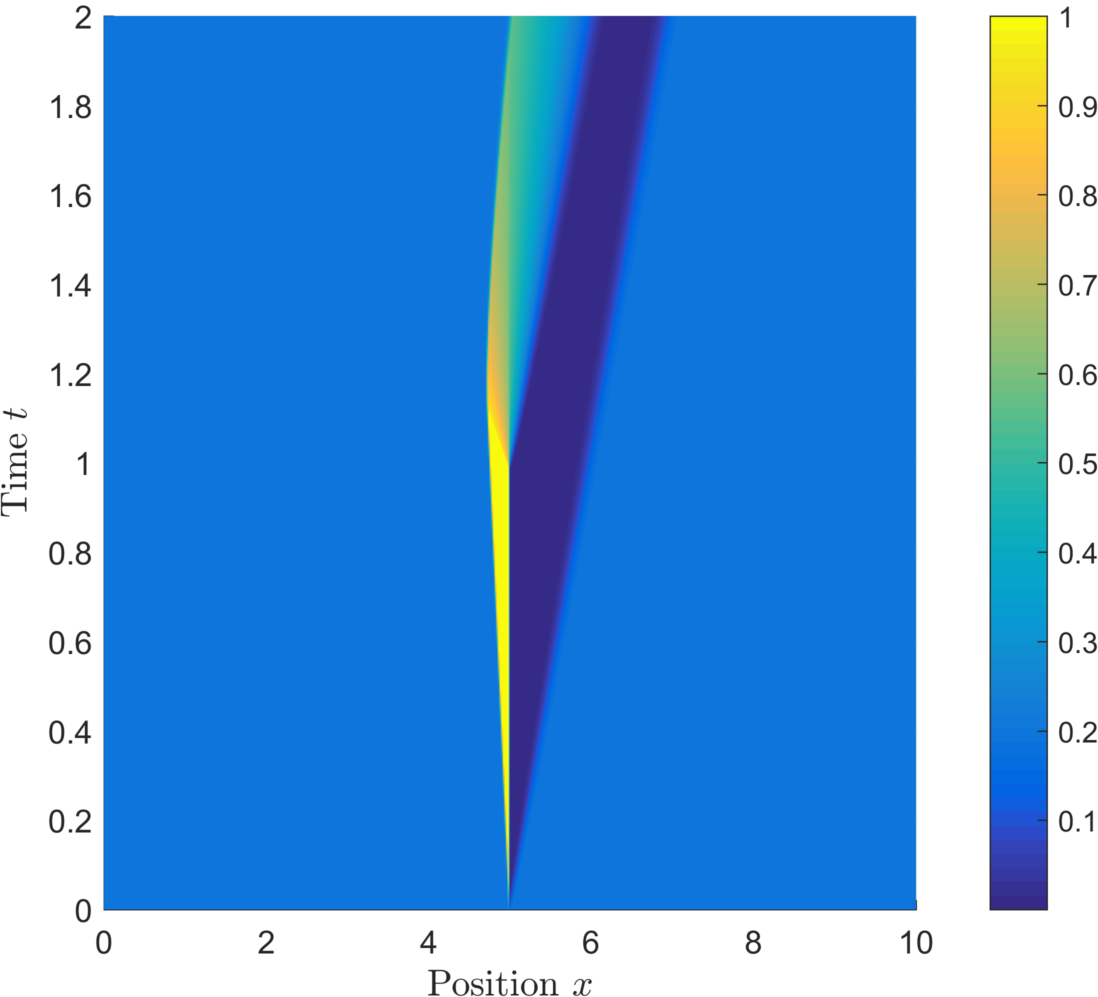
\includegraphics[width=0.75\textwidth]{1b_light_surf.png}
  \caption{Heatmap of $\rho(x,t)$ for light traffic: $\rho(0,t) = 0.2\rho_\mathrm{max}$.}
  \label{fig:1b_light_surf}
\end{figure}

\begin{figure}[h!]
  \centering
  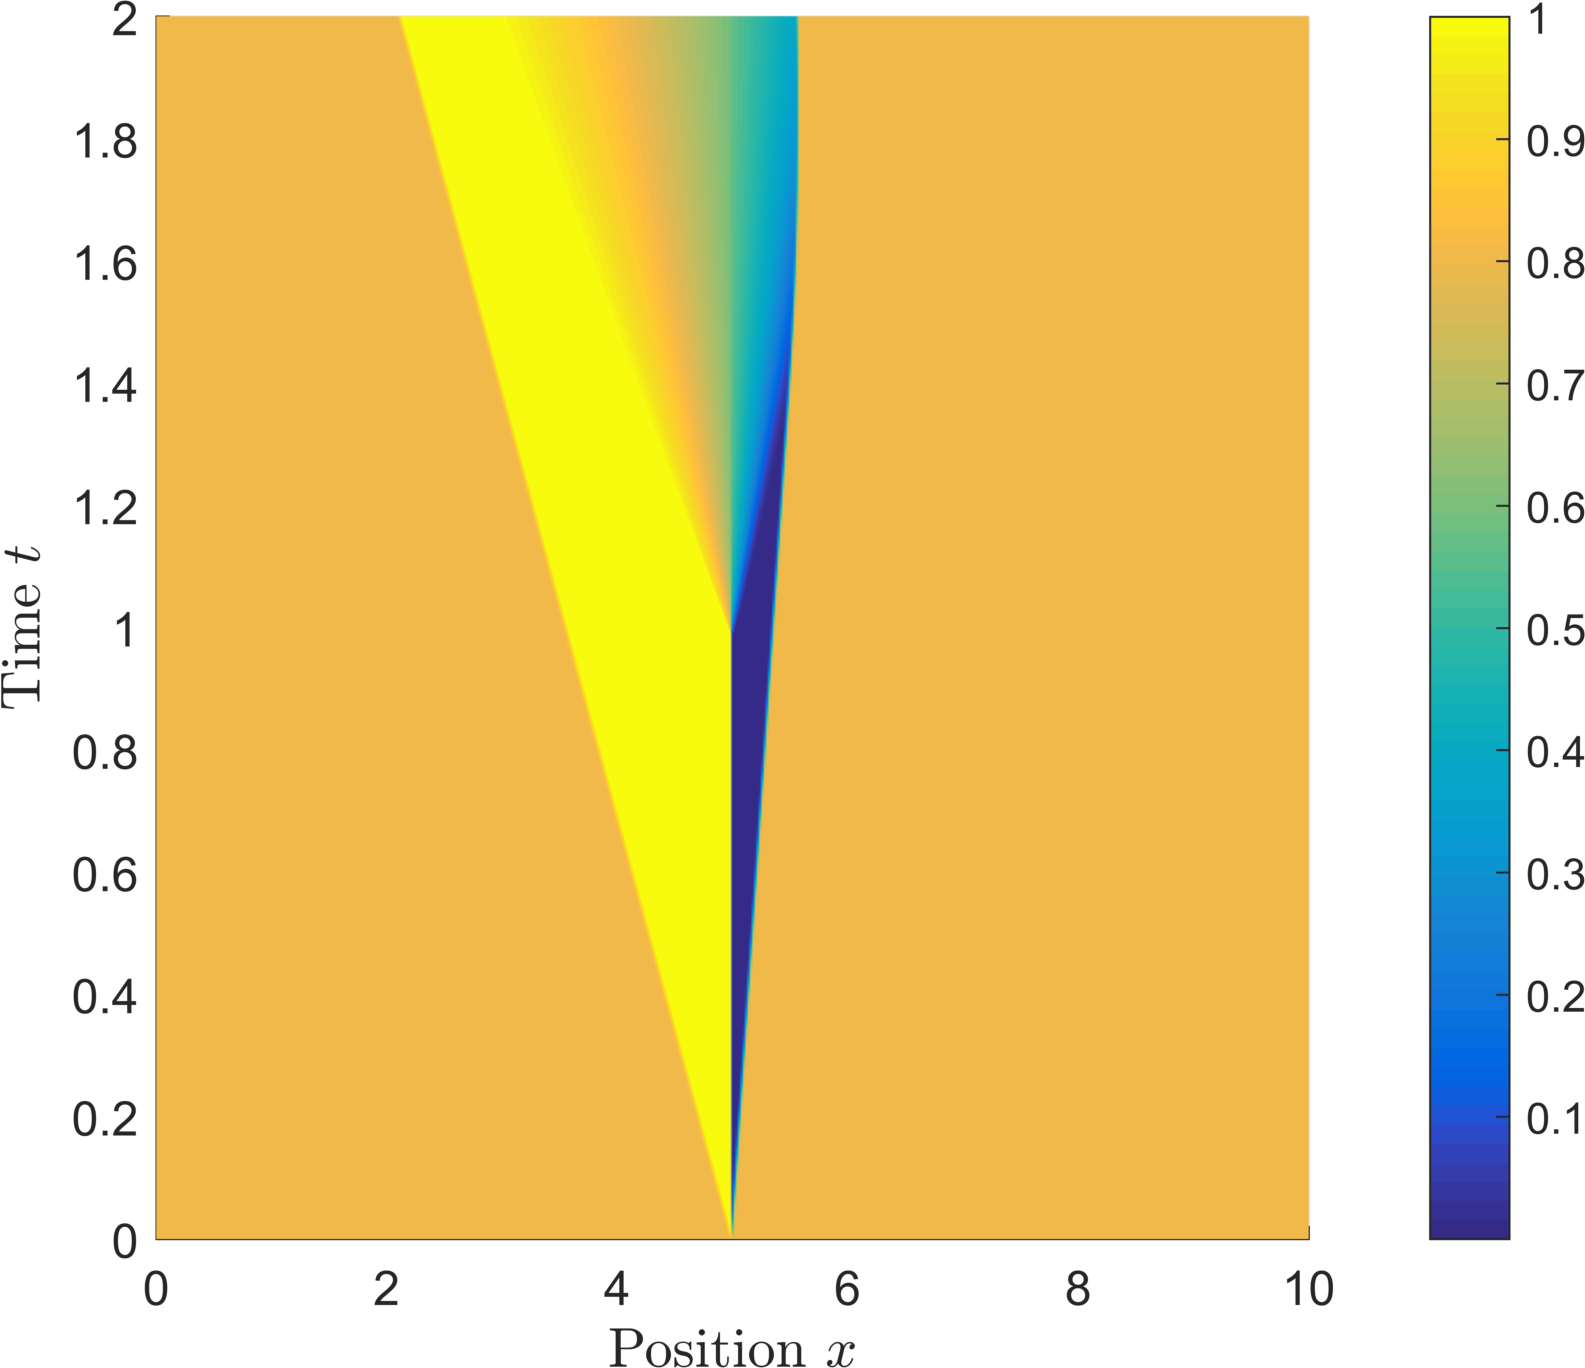
\includegraphics[width=0.75\textwidth]{1b_heavy_surf.png}
  \caption{Heatmap of $\rho(x,t)$ for heavy traffic: $\rho(0,t) = 0.8\rho_\mathrm{max}$.}
  \label{fig:1b_heavy_surf}
\end{figure}

% Question 2a

\begin{figure}[h!]
  \centering
  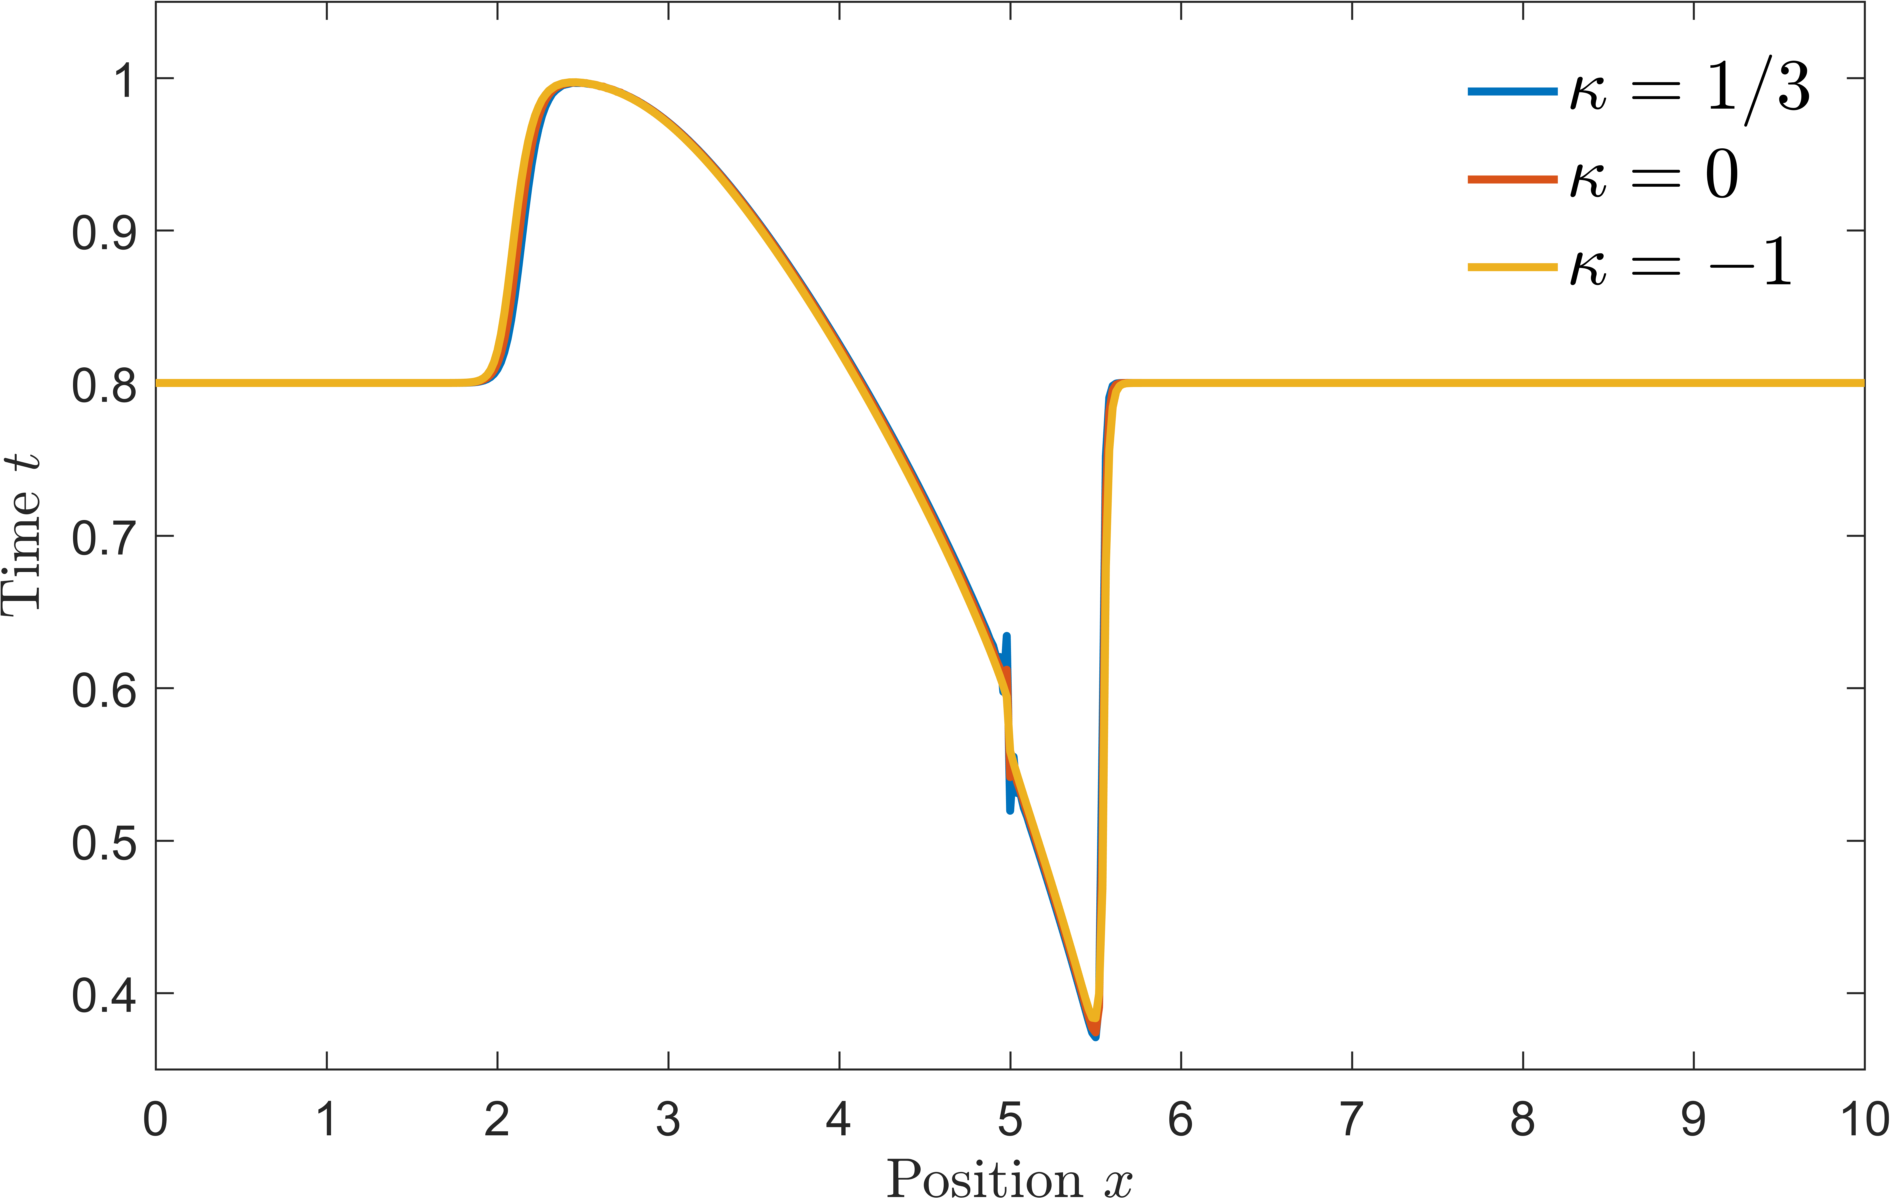
\includegraphics[width=\textwidth]{2a_heavy.png}
  \caption{}
  \label{fig:2a_heavy}
\end{figure}

\begin{figure}[h!]
  \centering
  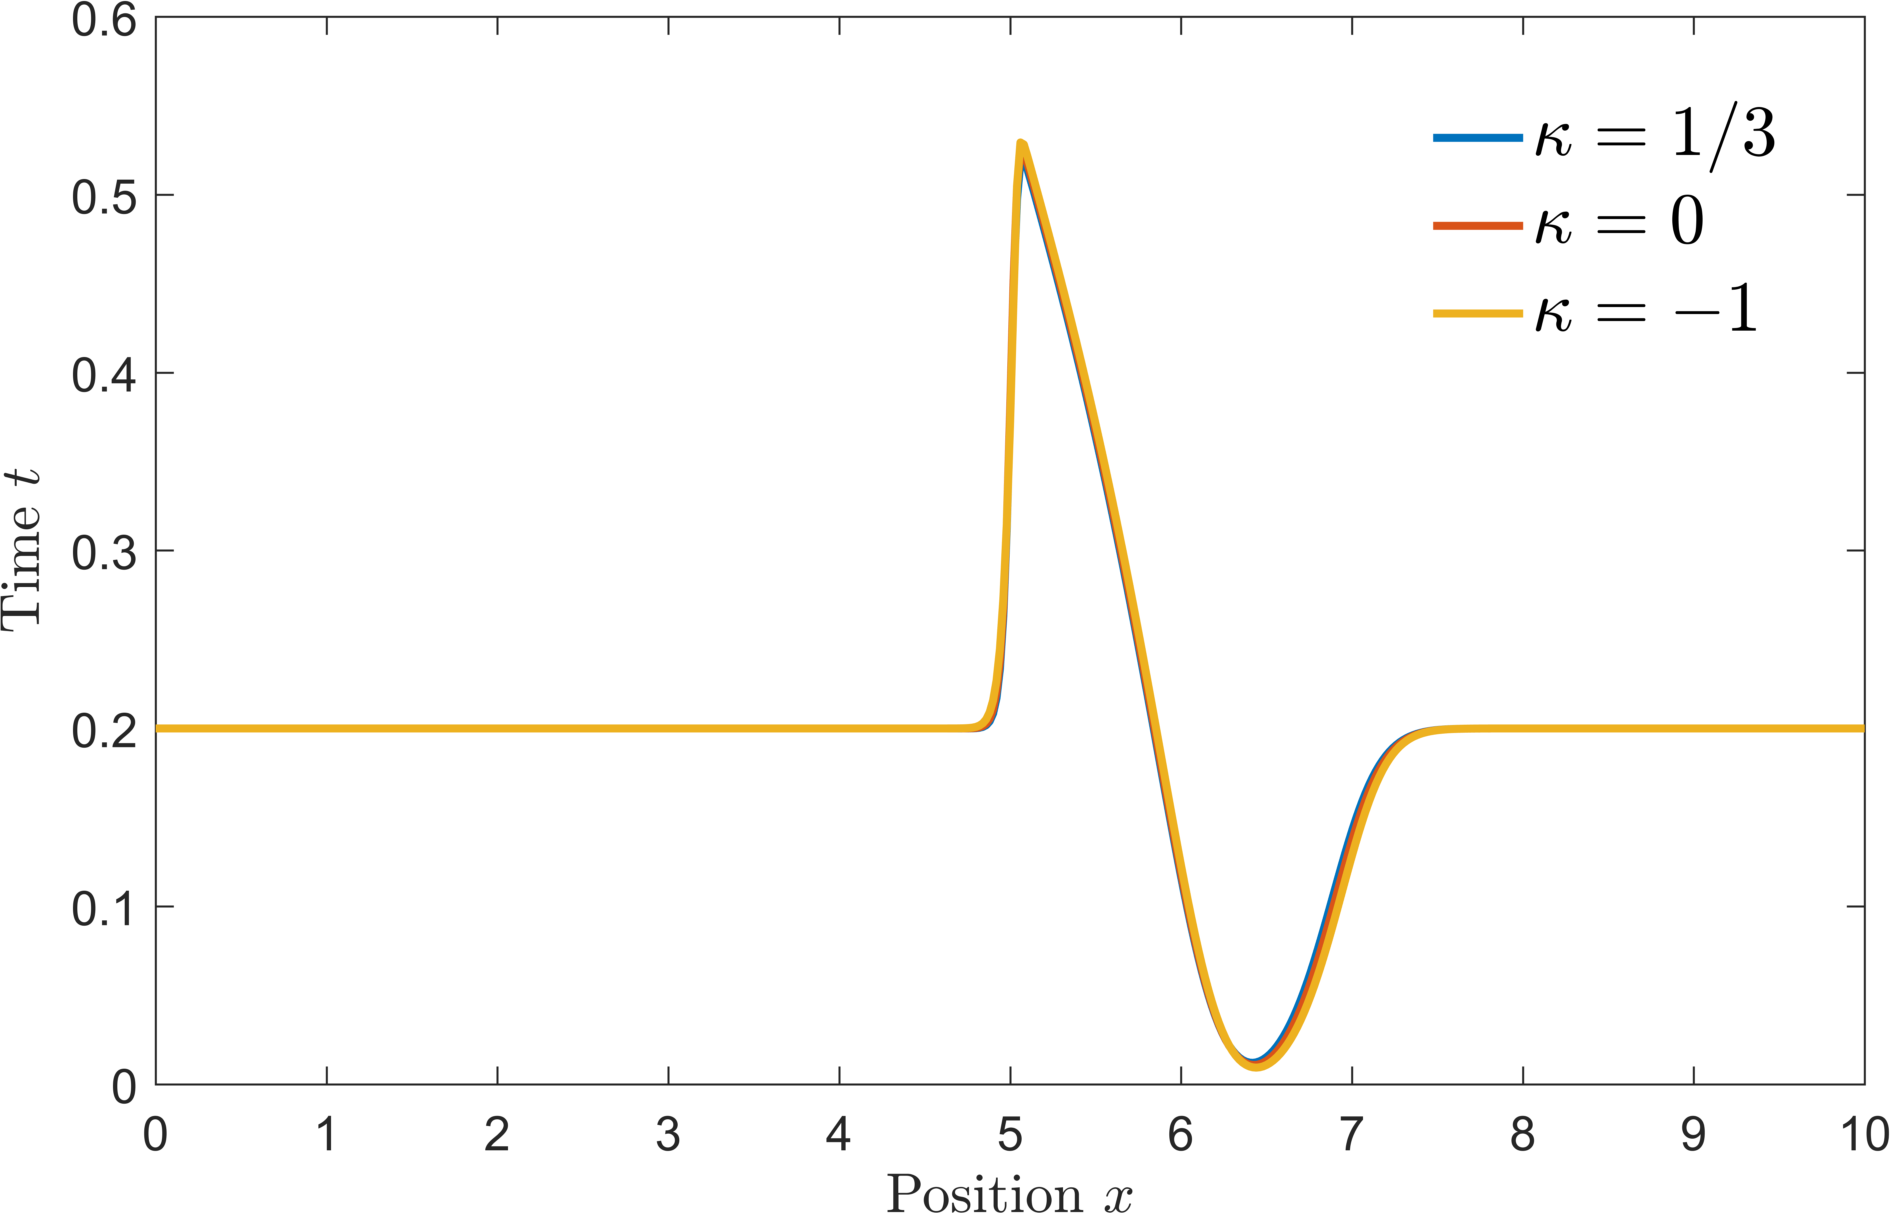
\includegraphics[width=\textwidth]{2a_light.png}
  \caption{}
  \label{fig:2a_light}
\end{figure}

% Question 2b

The minmod scheme $\phi(r) = \max\left\{ 0, \min\left\{r,1\right\} \right\}$. 
Superbee $\phi(r) = \max \left\{ 0, \min\left\{2r,1\right\}, \min\left\{r,2\right\} \right\} $.
van Leer $\displaystyle \phi(r) = \frac{r + |r|}{1 + |r|}$.

\begin{figure}[h!]
  \centering
  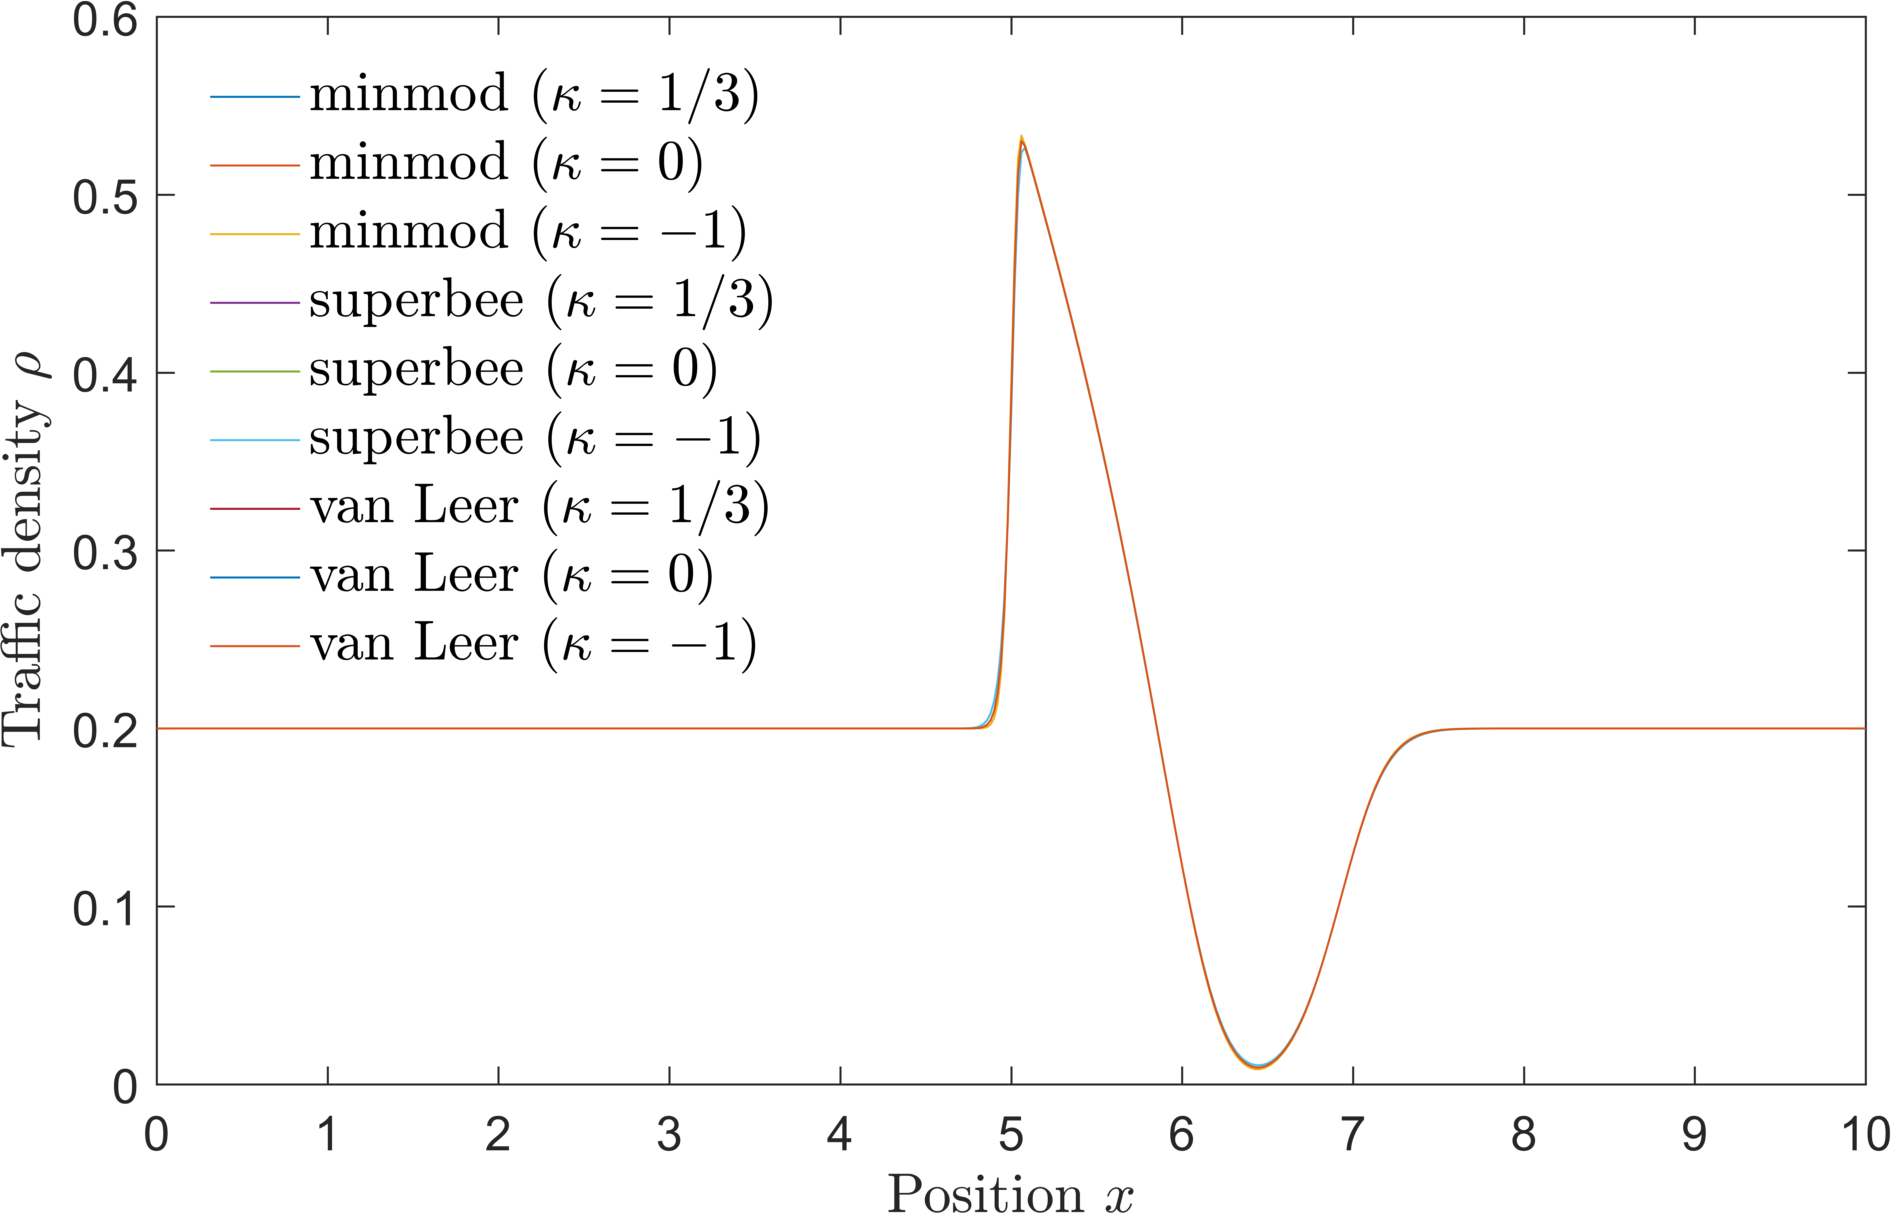
\includegraphics[width=\textwidth]{2b_all.png}
  \caption{}
  \label{fig:2b_all}
\end{figure}


\end{document}